
%(BEGIN_QUESTION)
% Copyright 2006, Tony R. Kuphaldt, released under the Creative Commons Attribution License (v 1.0)
% This means you may do almost anything with this work of mine, so long as you give me proper credit

Some differential pressure transmitters are equipped with {\it five-valve manifolds}.  These valve networks allow for blocking, equalizing, and bleeding of the transmitter's two pressure ports, the valves being arranged in this pattern:

$$\includegraphics[width=15.5cm]{i00212x01.eps}$$

Shown using standard P\&ID (Process and Instrument Diagram) symbols -- instrumentation equivalent of an electrical schematic diagram -- the transmitter and manifold arrangement looks like this:

$$\includegraphics[width=15.5cm]{i00212x02.eps}$$

Identify the normal, operating valve positions (open/closed) for a five-valve manifold.  Describe the proper sequence of manifold valve operation to successfully prepare the transmitter for removal from the process.

\vskip 10pt

Why do you think we have such things as 5-valve manifolds?  What can be done with this manifold that cannot be done with a three-valve manifold?

\underbar{file i00212}
%(END_QUESTION)





%(BEGIN_ANSWER)

Normal valve positions:

\medskip
{\item{} Both block valves open.
{\item{} Both equalizing valves closed.
{\item{} Vent valve closed.
\medskip

\vskip 10pt

Removing differential pressure transmitter from service:

\medskip
{\item{} Close one block valve.
{\item{} Open both equalizing valves (which one first does not matter).
{\item{} Close the other block valve.
{\item{} Open the vent valve.
{\item{} Tag all valves, notifying of transmitter's planned return time/date.
{\item{} Disconnect the transmitter from the manifold.
\medskip

\vskip 10pt

Restoring the transmitter back to service is as simple as reversing all the steps taken to remove it from service (i.e. go through the list backwards, doing the reverse of each instruction).

One feature that 5-valve manifolds provide over 3-valve manifolds is the ability to route a vent tube to a remote (safer) location, for use with particularly hazardous process fluids.

5-valve manifolds allow for in-place transmitter calibration, provided one of the $\Delta$P transmitter's sides has an atmospheric vent.  By connecting the calibrating pressure source to the vent line, one can route the calibrating pressure to either side of the transmitter (only), while keeping the other side vented.

%(END_ANSWER)





%(BEGIN_NOTES)


%INDEX% Safety, isolation valves: 5-valve equalizing manifold

%(END_NOTES)


